\documentclass[twoside]{book}

% Packages required by doxygen
\usepackage{fixltx2e}
\usepackage{calc}
\usepackage{doxygen}
\usepackage[export]{adjustbox} % also loads graphicx
\usepackage{graphicx}
\usepackage[utf8]{inputenc}
\usepackage{makeidx}
\usepackage{multicol}
\usepackage{multirow}
\PassOptionsToPackage{warn}{textcomp}
\usepackage{textcomp}
\usepackage[nointegrals]{wasysym}
\usepackage[table]{xcolor}

% Font selection
\usepackage[T1]{fontenc}
\usepackage[scaled=.90]{helvet}
\usepackage{courier}
\usepackage{amssymb}
\usepackage{sectsty}
\renewcommand{\familydefault}{\sfdefault}
\allsectionsfont{%
  \fontseries{bc}\selectfont%
  \color{darkgray}%
}
\renewcommand{\DoxyLabelFont}{%
  \fontseries{bc}\selectfont%
  \color{darkgray}%
}
\newcommand{\+}{\discretionary{\mbox{\scriptsize$\hookleftarrow$}}{}{}}

% Page & text layout
\usepackage{geometry}
\geometry{%
  a4paper,%
  top=2.5cm,%
  bottom=2.5cm,%
  left=2.5cm,%
  right=2.5cm%
}
\tolerance=750
\hfuzz=15pt
\hbadness=750
\setlength{\emergencystretch}{15pt}
\setlength{\parindent}{0cm}
\setlength{\parskip}{0.2cm}
\makeatletter
\renewcommand{\paragraph}{%
  \@startsection{paragraph}{4}{0ex}{-1.0ex}{1.0ex}{%
    \normalfont\normalsize\bfseries\SS@parafont%
  }%
}
\renewcommand{\subparagraph}{%
  \@startsection{subparagraph}{5}{0ex}{-1.0ex}{1.0ex}{%
    \normalfont\normalsize\bfseries\SS@subparafont%
  }%
}
\makeatother

% Headers & footers
\usepackage{fancyhdr}
\pagestyle{fancyplain}
\fancyhead[LE]{\fancyplain{}{\bfseries\thepage}}
\fancyhead[CE]{\fancyplain{}{}}
\fancyhead[RE]{\fancyplain{}{\bfseries\leftmark}}
\fancyhead[LO]{\fancyplain{}{\bfseries\rightmark}}
\fancyhead[CO]{\fancyplain{}{}}
\fancyhead[RO]{\fancyplain{}{\bfseries\thepage}}
\fancyfoot[LE]{\fancyplain{}{}}
\fancyfoot[CE]{\fancyplain{}{}}
\fancyfoot[RE]{\fancyplain{}{\bfseries\scriptsize Generated on Sat Nov 14 2015 21\+:17\+:22 for A2 by Doxygen }}
\fancyfoot[LO]{\fancyplain{}{\bfseries\scriptsize Generated on Sat Nov 14 2015 21\+:17\+:22 for A2 by Doxygen }}
\fancyfoot[CO]{\fancyplain{}{}}
\fancyfoot[RO]{\fancyplain{}{}}
\renewcommand{\footrulewidth}{0.4pt}
\renewcommand{\chaptermark}[1]{%
  \markboth{#1}{}%
}
\renewcommand{\sectionmark}[1]{%
  \markright{\thesection\ #1}%
}

% Indices & bibliography
\usepackage{natbib}
\usepackage[titles]{tocloft}
\setcounter{tocdepth}{3}
\setcounter{secnumdepth}{5}
\makeindex

% Hyperlinks (required, but should be loaded last)
\usepackage{ifpdf}
\ifpdf
  \usepackage[pdftex,pagebackref=true]{hyperref}
\else
  \usepackage[ps2pdf,pagebackref=true]{hyperref}
\fi
\hypersetup{%
  colorlinks=true,%
  linkcolor=blue,%
  citecolor=blue,%
  unicode%
}

% Custom commands
\newcommand{\clearemptydoublepage}{%
  \newpage{\pagestyle{empty}\cleardoublepage}%
}


%===== C O N T E N T S =====

\begin{document}

% Titlepage & ToC
\hypersetup{pageanchor=false,
             bookmarks=true,
             bookmarksnumbered=true,
             pdfencoding=unicode
            }
\pagenumbering{roman}
\begin{titlepage}
\vspace*{7cm}
\begin{center}%
{\Large A2 }\\
\vspace*{1cm}
{\large Generated by Doxygen 1.8.10}\\
\vspace*{0.5cm}
{\small Sat Nov 14 2015 21:17:22}\\
\end{center}
\end{titlepage}
\clearemptydoublepage
\tableofcontents
\clearemptydoublepage
\pagenumbering{arabic}
\hypersetup{pageanchor=true}

%--- Begin generated contents ---
\chapter{A2}
\label{md__r_e_a_d_m_e}
\hypertarget{md__r_e_a_d_m_e}{}
S\+E\+N\+G330\+A2 
\chapter{Hierarchical Index}
\section{Class Hierarchy}
This inheritance list is sorted roughly, but not completely, alphabetically\+:\begin{DoxyCompactList}
\item \contentsline{section}{Equipment}{\pageref{class_equipment}}{}
\begin{DoxyCompactList}
\item \contentsline{section}{Bike}{\pageref{class_bike}}{}
\item \contentsline{section}{Tread\+Mill}{\pageref{class_tread_mill}}{}
\end{DoxyCompactList}
\item \contentsline{section}{Equipment\+Manager}{\pageref{class_equipment_manager}}{}
\end{DoxyCompactList}

\chapter{Class Index}
\section{Class List}
Here are the classes, structs, unions and interfaces with brief descriptions\+:\begin{DoxyCompactList}
\item\contentsline{section}{\hyperlink{class_bike}{Bike} }{\pageref{class_bike}}{}
\item\contentsline{section}{\hyperlink{class_equipment}{Equipment} }{\pageref{class_equipment}}{}
\item\contentsline{section}{\hyperlink{class_equipment_manager}{Equipment\+Manager} }{\pageref{class_equipment_manager}}{}
\item\contentsline{section}{\hyperlink{class_tread_mill}{Tread\+Mill} }{\pageref{class_tread_mill}}{}
\end{DoxyCompactList}

\chapter{Class Documentation}
\hypertarget{class_bike}{}\section{Bike Class Reference}
\label{class_bike}\index{Bike@{Bike}}
Inheritance diagram for Bike\+:\begin{figure}[H]
\begin{center}
\leavevmode
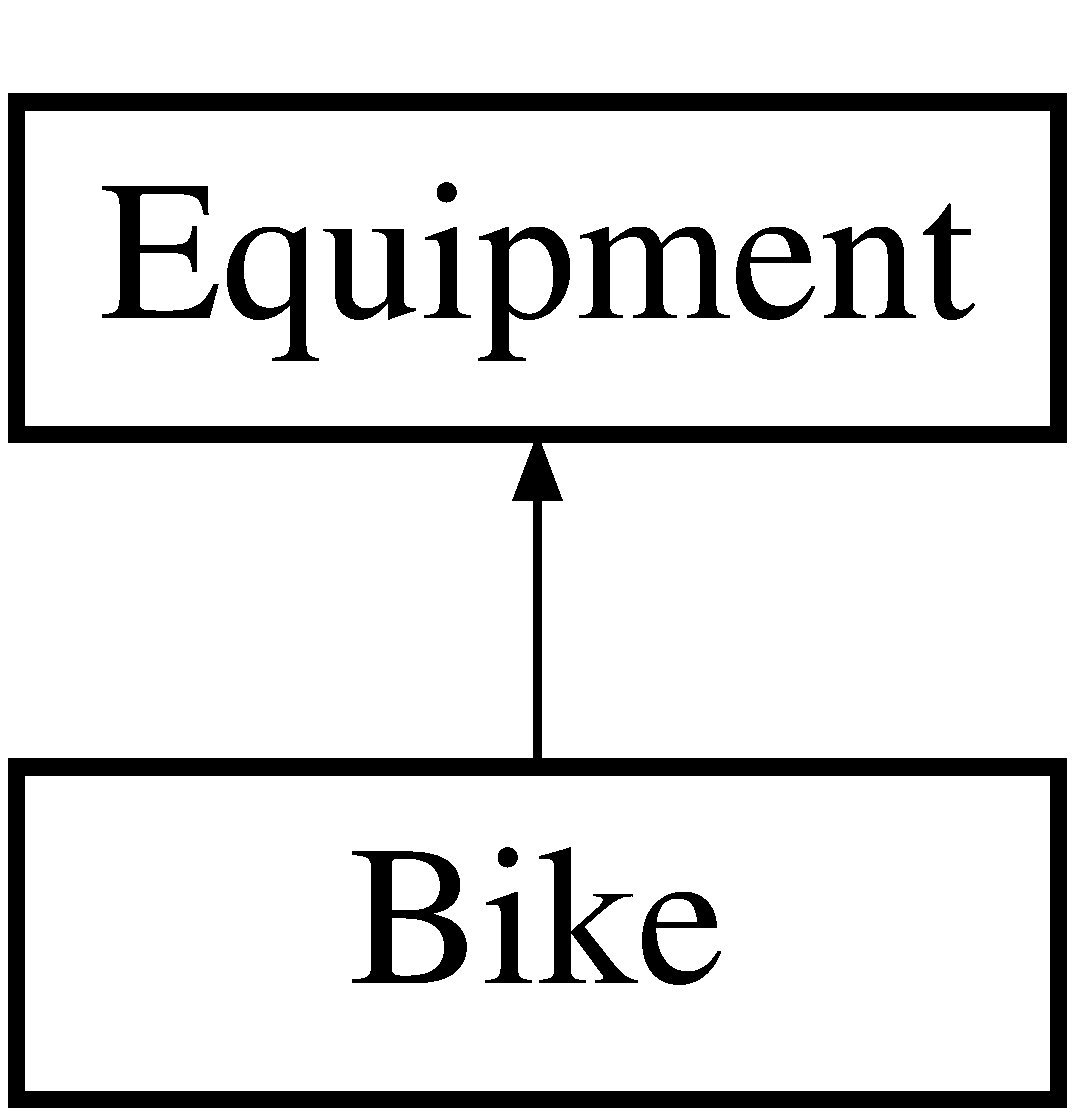
\includegraphics[height=2.000000cm]{class_bike}
\end{center}
\end{figure}
\subsection*{Public Member Functions}
\begin{DoxyCompactItemize}
\item 
\hyperlink{class_bike_a96d2a8bb51ae3901533e6bdd26d30916}{Bike} (string name)
\item 
\hypertarget{class_bike_aea282b61c87845ec59e5483ca2601b2d}{}{\bfseries Bike} (const \hyperlink{class_bike}{Bike} \&bike)\label{class_bike_aea282b61c87845ec59e5483ca2601b2d}

\item 
\hypertarget{class_bike_ae7010c424ae4a33f7ec03b4292aa7807}{}\hyperlink{class_equipment}{Equipment} $\ast$ {\bfseries clone} ()\label{class_bike_ae7010c424ae4a33f7ec03b4292aa7807}

\item 
\hypertarget{class_bike_ab57533db1d20e084f4e86e3d295635e2}{}void {\bfseries display} () const \label{class_bike_ab57533db1d20e084f4e86e3d295635e2}

\item 
\hypertarget{class_bike_a3bb418d8f5495341819aa91667bf68a5}{}void {\bfseries set\+Name} (string name)\label{class_bike_a3bb418d8f5495341819aa91667bf68a5}

\end{DoxyCompactItemize}


\subsection{Constructor \& Destructor Documentation}
\hypertarget{class_bike_a96d2a8bb51ae3901533e6bdd26d30916}{}\index{Bike@{Bike}!Bike@{Bike}}
\index{Bike@{Bike}!Bike@{Bike}}
\subsubsection[{Bike(string name)}]{\setlength{\rightskip}{0pt plus 5cm}Bike\+::\+Bike (
\begin{DoxyParamCaption}
\item[{string}]{name}
\end{DoxyParamCaption}
)\hspace{0.3cm}{\ttfamily [inline]}}\label{class_bike_a96d2a8bb51ae3901533e6bdd26d30916}
\hyperlink{class_bike}{Bike} sub class of \hyperlink{class_equipment}{Equipment} has a type and name 

The documentation for this class was generated from the following file\+:\begin{DoxyCompactItemize}
\item 
A2/\+A2/Equipment.\+cpp\end{DoxyCompactItemize}

\hypertarget{class_equipment}{}\section{Equipment Class Reference}
\label{class_equipment}\index{Equipment@{Equipment}}
Inheritance diagram for Equipment\+:\begin{figure}[H]
\begin{center}
\leavevmode
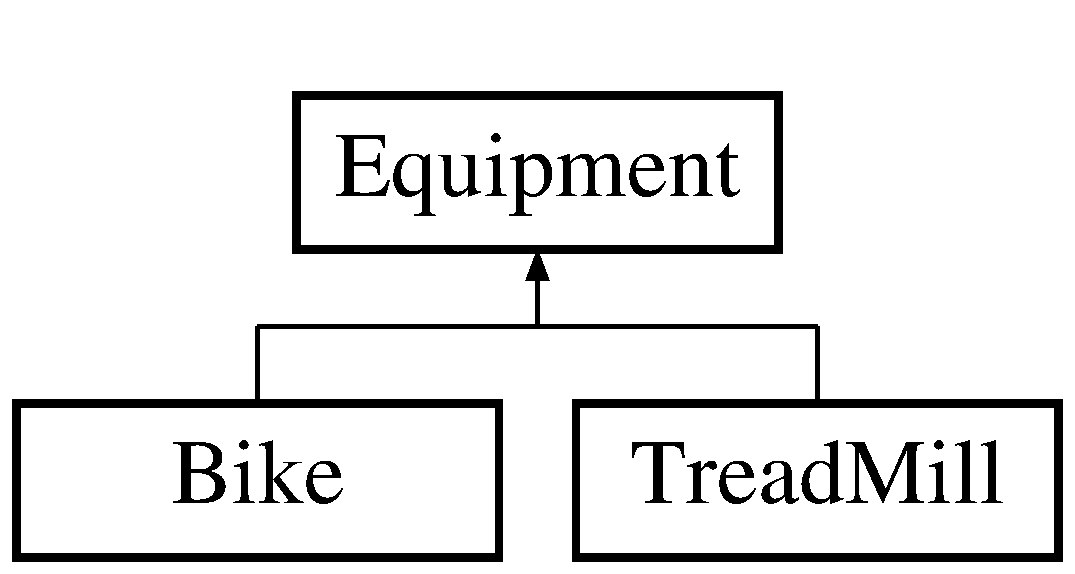
\includegraphics[height=2.000000cm]{class_equipment}
\end{center}
\end{figure}
\subsection*{Public Member Functions}
\begin{DoxyCompactItemize}
\item 
\hyperlink{class_equipment_a2bd67c4254f2074f4f7469f29a20e760}{Equipment} ()
\item 
\hypertarget{class_equipment_a866383329b92e50a2c323e05e55fa948}{}virtual \hyperlink{class_equipment}{Equipment} $\ast$ {\bfseries clone} ()=0\label{class_equipment_a866383329b92e50a2c323e05e55fa948}

\item 
\hypertarget{class_equipment_a57a1aab4d84f6ac375e62b34f77d113e}{}virtual void {\bfseries display} () const  =0\label{class_equipment_a57a1aab4d84f6ac375e62b34f77d113e}

\item 
\hypertarget{class_equipment_afe20b9aaf51fb4d6aff61157310d33da}{}virtual void {\bfseries set\+Name} (string)=0\label{class_equipment_afe20b9aaf51fb4d6aff61157310d33da}

\end{DoxyCompactItemize}


\subsection{Constructor \& Destructor Documentation}
\hypertarget{class_equipment_a2bd67c4254f2074f4f7469f29a20e760}{}\index{Equipment@{Equipment}!Equipment@{Equipment}}
\index{Equipment@{Equipment}!Equipment@{Equipment}}
\subsubsection[{Equipment()}]{\setlength{\rightskip}{0pt plus 5cm}Equipment\+::\+Equipment (
\begin{DoxyParamCaption}
{}
\end{DoxyParamCaption}
)\hspace{0.3cm}{\ttfamily [inline]}}\label{class_equipment_a2bd67c4254f2074f4f7469f29a20e760}
\hyperlink{class_equipment}{Equipment} virtual class 

The documentation for this class was generated from the following file\+:\begin{DoxyCompactItemize}
\item 
A2/\+A2/Equipment.\+cpp\end{DoxyCompactItemize}

\hypertarget{class_equipment_manager}{}\section{Equipment\+Manager Class Reference}
\label{class_equipment_manager}\index{Equipment\+Manager@{Equipment\+Manager}}
\subsection*{Public Member Functions}
\begin{DoxyCompactItemize}
\item 
\hyperlink{class_equipment_manager_acc90b089a43958a1c94c5a0d900b452f}{Equipment\+Manager} ()
\item 
\hypertarget{class_equipment_manager_ad20977fa533bf61eedc6b3f945754dee}{}\hyperlink{class_equipment}{Equipment} $\ast$ {\bfseries create\+Equipment} (eq\+Type type)\label{class_equipment_manager_ad20977fa533bf61eedc6b3f945754dee}

\end{DoxyCompactItemize}


\subsection{Constructor \& Destructor Documentation}
\hypertarget{class_equipment_manager_acc90b089a43958a1c94c5a0d900b452f}{}\index{Equipment\+Manager@{Equipment\+Manager}!Equipment\+Manager@{Equipment\+Manager}}
\index{Equipment\+Manager@{Equipment\+Manager}!Equipment\+Manager@{Equipment\+Manager}}
\subsubsection[{Equipment\+Manager()}]{\setlength{\rightskip}{0pt plus 5cm}Equipment\+Manager\+::\+Equipment\+Manager (
\begin{DoxyParamCaption}
{}
\end{DoxyParamCaption}
)\hspace{0.3cm}{\ttfamily [inline]}}\label{class_equipment_manager_acc90b089a43958a1c94c5a0d900b452f}
\hyperlink{class_equipment_manager}{Equipment\+Manager} used to create and manage clones 

The documentation for this class was generated from the following file\+:\begin{DoxyCompactItemize}
\item 
A2/\+A2/Equipment.\+cpp\end{DoxyCompactItemize}

\hypertarget{class_tread_mill}{}\section{Tread\+Mill Class Reference}
\label{class_tread_mill}\index{Tread\+Mill@{Tread\+Mill}}
Inheritance diagram for Tread\+Mill\+:\begin{figure}[H]
\begin{center}
\leavevmode
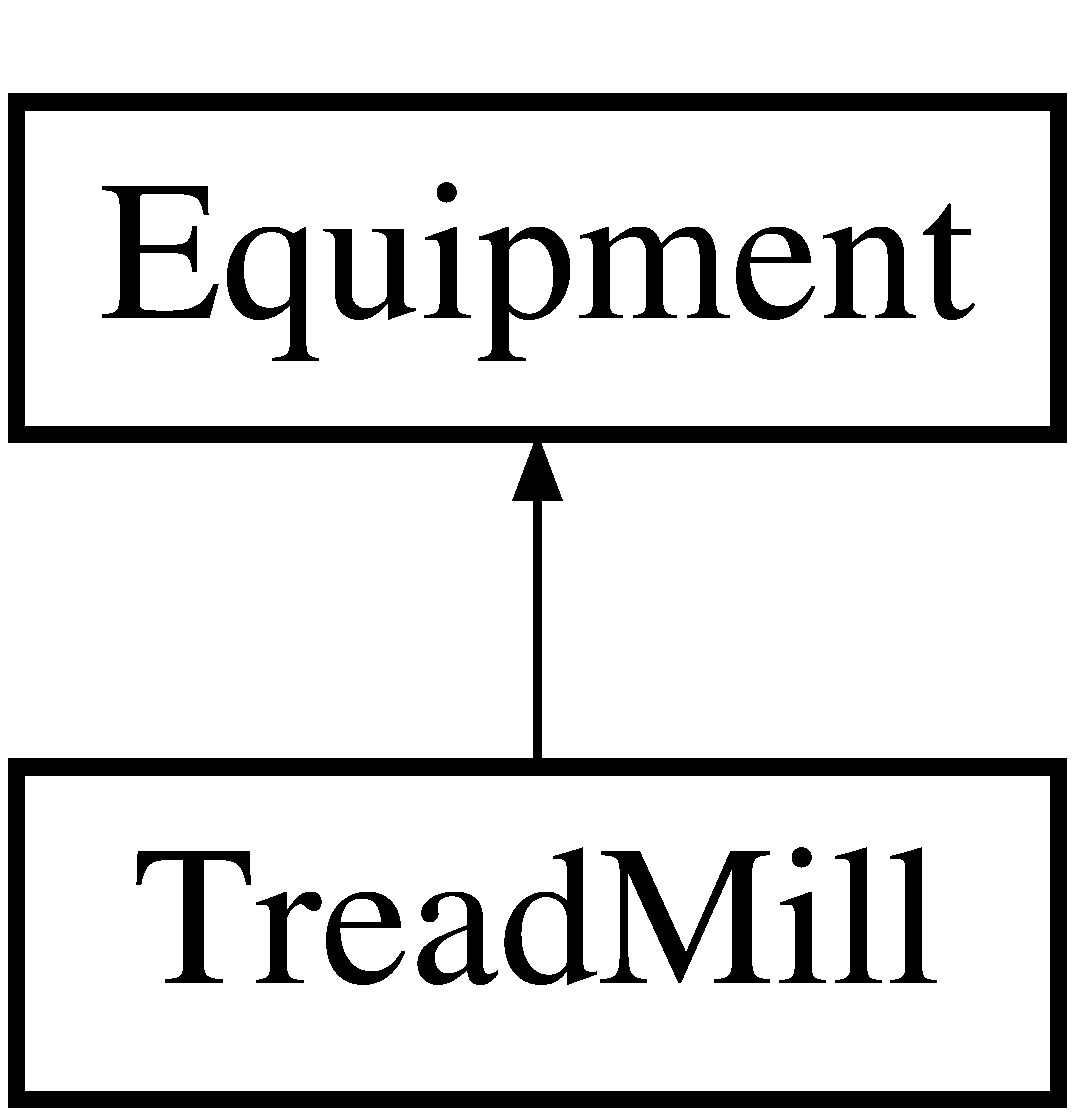
\includegraphics[height=2.000000cm]{class_tread_mill}
\end{center}
\end{figure}
\subsection*{Public Member Functions}
\begin{DoxyCompactItemize}
\item 
\hyperlink{class_tread_mill_afd39fc1fd5b86d32163c5e3d19477f0a}{Tread\+Mill} (string name)
\item 
\hypertarget{class_tread_mill_aa018f889df4fefdd7f855de4743eed09}{}{\bfseries Tread\+Mill} (const \hyperlink{class_tread_mill}{Tread\+Mill} \&tread)\label{class_tread_mill_aa018f889df4fefdd7f855de4743eed09}

\item 
\hypertarget{class_tread_mill_a87e09b167ded580bc92e13e05ad8e2ef}{}\hyperlink{class_equipment}{Equipment} $\ast$ {\bfseries clone} ()\label{class_tread_mill_a87e09b167ded580bc92e13e05ad8e2ef}

\item 
\hypertarget{class_tread_mill_ac0ebca20ccdd0e5563473d5c6408bb6f}{}void {\bfseries display} () const \label{class_tread_mill_ac0ebca20ccdd0e5563473d5c6408bb6f}

\item 
\hypertarget{class_tread_mill_a42d59ef0a32ec6ac6f9401d91230cb21}{}void {\bfseries set\+Name} (string name)\label{class_tread_mill_a42d59ef0a32ec6ac6f9401d91230cb21}

\end{DoxyCompactItemize}


\subsection{Constructor \& Destructor Documentation}
\hypertarget{class_tread_mill_afd39fc1fd5b86d32163c5e3d19477f0a}{}\index{Tread\+Mill@{Tread\+Mill}!Tread\+Mill@{Tread\+Mill}}
\index{Tread\+Mill@{Tread\+Mill}!Tread\+Mill@{Tread\+Mill}}
\subsubsection[{Tread\+Mill(string name)}]{\setlength{\rightskip}{0pt plus 5cm}Tread\+Mill\+::\+Tread\+Mill (
\begin{DoxyParamCaption}
\item[{string}]{name}
\end{DoxyParamCaption}
)\hspace{0.3cm}{\ttfamily [inline]}}\label{class_tread_mill_afd39fc1fd5b86d32163c5e3d19477f0a}
Treadmill sub class of \hyperlink{class_equipment}{Equipment} has a type and name 

The documentation for this class was generated from the following file\+:\begin{DoxyCompactItemize}
\item 
A2/\+A2/Equipment.\+cpp\end{DoxyCompactItemize}

%--- End generated contents ---

% Index
\backmatter
\newpage
\phantomsection
\clearemptydoublepage
\addcontentsline{toc}{chapter}{Index}
\printindex

\end{document}
